\chapter{THE PACKET PIPELINE PROCESSING MODEL} \label{ch:pipeline_model}

Steve uses a \textit{pipeline processing model} to process packets. The pipeline processing model is a series of \textit{data processing stages}. Each stage is connected to the next in such a way that the output of one stage becomes the input to the next. These stages will decode the packet, modify the packet, and ultimately decide which port to forward the packet on.

A Steve pipeline can be described in terms of four phases: 1) \textit{ingress processing}, 2) \textit{decoding stages}, 3) \textit{table matching stages}, and 4) \textit{egress processing}. Of these four phases, decoding and table matching are our two kinds of data processing stages. Figure \ref{fg:pipeline_model} demonstrates the flow of packets through Steve's pipeline. This chapter will describe each of these phases.

\begin{figure}
\caption{The flow of a packet through the Steve pipeline. The first phase is ingress processing, where a \textit{context} (described in Section \ref{context_desc}) is built around the packet. Then a number of decoding and table matching stages may decode, modify, and make forwarding decisions on the packet. Lastly, the packet goes through egress processing, where it is ultimately forwarded (or dropped).}
\label{fg:pipeline_model}
\end{figure}

The Steve programming language allows programmers to define what \textit{decoding} and \textit{table matching} stages do and how they are connected. Keep in mind that the pipeline processing model is essentially a state machine. Each processing stage is a state in the machine. Each state has a set of conditions which, when met, causes the packet to move to new stages, or new states. This can be represented as a graph where each processing stage is a node on the graph and each stage is connected to the next with an edge. This is a valuable property as it allows the Steve programming language to analyze these pipelines and enforce certain logical, safety, and correctness guarantees about a user-defined pipeline.

Steve pipelines follow a run-to-complete model of execution. Once a packet enters the pipeline, each processing stage is consecutively applied to the packet. Once no more stages are applied through program logic, the packet exits the pipeline.

\subsection{Ingress Processing} \label{ingress_desc}

A packet enters a network device on a port, known as its \textit{ingress port}. At this time, the data plane builds a data structure known as the \textit{context} is built around the packet. This context is what the pipeline uses to save data as the packet moves through the pipeline. Further explanation of the context can be found in Section \ref{context_desc}.

After ingress processing, the data plane dispatches the context (which includes the packet) to the first decoding stage.

The ingress processing stage is not something that is written in a Steve application. It is implicit and handled by the Flowpath data plane discussed in Chapter \ref{ch:flowpath}. 

\subsection{Packet Context} \label{context_desc}

Pipeline stages are connected in such a way that the output from one stage becomes the input to the next. The \textit{context} data structure is that output and input. It carries data between stages. A stage often needs to use data created by prior stages. As a packet moves between stages, information such as the position and length of extracted fields and headers must be saved for later recovery. To save this information, Steve applications use a data structure called the packet \textbf{context}. Specifically, a Steve context saves the following data:

\begin{itemize}
\item The packet itself. From now on, anytime mention of the context is made, it is implied that this also includes the packet itself.
\item The packet's logical and physical ingress ports.
\item The packet's length.
\item A tunnel identifier.
\item The offset and length of decoded fields.
\item The offset of decoded headers.
\item An action set that may be written to and is executed during egress processing.
\end{itemize}

Extracted fields and headers get saved in \textbf{binding environments} contained within the context. The term \textbf{environment} refers to a structure which maps names (in this case field and header names) to their storage location during runtime \cite{compilers1}. The mapping of those storage locations to the values held there is known as \textbf{state}. There is a binding environment for fields and headers respectively.

Figure \ref{fg:ContextEnv} depicts the binding environment. The field binding environment is used to map fields to offset-length pairs where that field can be found. The header binding environment similarly maps headers to offsets where that header can be found. These mappings are known as \textit{bindings}.

\begin{figure}
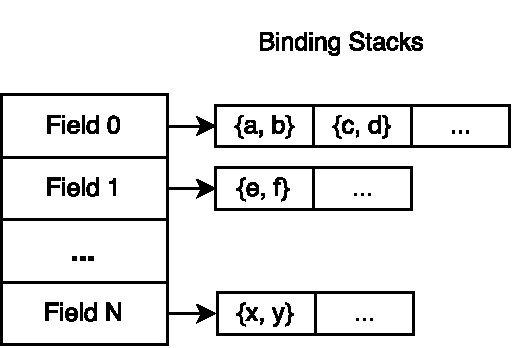
\includegraphics[scale=0.75,natwidth=203,natheight=298]{context}
\caption{The binding environment inside a context used to store the length and offset of fields, or the offset of headers. On the left, indexes one through sixteen represent the fields that can be extracted. Each field maintains a binding stack. Each element in the binding stack is a binding which stores the offset and length where an instance of that field can be found. }
\label{fg:ContextEnv}
\end{figure}

Since any given packet can contain one or more of any field or header with the same name, a binding environment maintains a stack for every field and header. These stacks are called \textit{binding stacks}. By extension, this means an environment is actually a mapping of field names to binding stacks. When the value of a field is needed, the topmost binding on the binding stack shall be used to recover the value of that field.

The implementation of a binding environment in Flowpath is a fixed-sized array where each element in the array is a fixed-sized binding stack. Each valid index in the array represents a unique field or header name extracted by the Steve application. The compiler is responsible for associating all unique field names to unique integer indexes. The same is done for all unique headers. This provides constant time lookup of field bindings without the overhead of hashing complex names.

Figure \ref{fg:ContextEnvWorking} demonstrates how data is stored in the context as it is being decoded. The example is a packet which contains an encapsulated IPv4 header commonly used in IP tunneling. In the ethernet decoding stage which extract the \texttt{src}, \texttt{dst}, and \texttt{type} field are extracted and stored in the context. Next we determine that IPv4 follows based on the \texttt{type} field. We extract IPv4 \texttt{dst} and \texttt{protocol}. The \texttt{protocol} field tells us we have another IPv4 header after the current one. We move to decode that and once again we extract IPv4 \texttt{dst} and \texttt{protocol}. Note how the new values of IPv4 are pushed on top of the binding stack. Any further usage of those fields will use the latest values extracted for those fields. Keep in mind that this means any usage of the first set of IPv4 \texttt{dst} and \texttt{protocol} must occur before the decoding of the second IPv4 header.\

\begin{figure}
TODO: Make an image for this.
\caption{A context environment in action during runtime.}
\label{fg:ContextEnvWorking}
\end{figure}

The \textbf{action set} is the other major data structure contained within the context. Actions are written to the action set for \textit{deferred execution} through the course of a pipeline. These actions are executed once the pipeline is complete, during the egress processing phase.

\section{Decoding Stage} \label{decoder_desc}

When a packet is received on its ingress port, it is a chunk of raw, uninterpreted data. Before a packet can be processed and routed, its headers and fields must be decoded and extracted so that meaningful decisions can be made about based on those values. The decoding stage is responsible for this.

Steve allows for programmers to specify \textit{how} and \textit{which} fields are extracted from headers. In other paradigms, the \textit{entire} packet is decoded from start to finish; all headers and all fields are extracted, then all fields are saved. This is what is considered a \textbf{full decode}. After this full decode, the decision making process on the packet begins using those saved fields. However, this method is inherently inefficient. Only certain fields and headers within a packet are ever really needed. To compound this, different devices may care about different subsets of fields within a given packet. Decoding all headers and fields from a packet is inherently wasteful.

Full decodes waste valuable processing time. Efficiency is important when dealing with networking equipment which has to processes between 10Gbps to 40Gbps. This inherent inefficiency is why Steve proposes the idea of a \textit{partial decode}. Unlike similar SDN-focused programming languages, Steve is designed to allow programmers to specify the extraction of only specific fields rather than an entire header. Though the specification may be verbose in some cases, it makes programmers think very carefully about which fields they need and which fields they do not. 

Additionally, Steve proposes that not all headers need to be decoded. For example, if a networking application only needs to forward using MAC addresses, there is no reason to waste time extracting fields from IPv4 or IPv6 headers, and so on.

That being said, Steve also supports the full decode. It may be desirable to some programmers to do this in certain scenarios, thus the language does not favor one paradigm over another.

\section{Table Stage} \label{table_desc}

Table stages handle matching against extracted fields, i.e. classification, and perform a sequence of desired actions on like-classified packets. This is done through a mechanism known as a flow table defined by the OpenFlow standard \cite{openflow_spec}.

A \textbf{flow table} is composed of a set of \textbf{flow entries}. A flow entry is composed of \textbf{match fields}, a \textbf{priority}, a set of \textbf{actions}, and miscellaneous additional data. Each table specifies a set of key fields that together make up a \textbf{key} for that table. For each key field, each flow entry has a corresponding value, known as a \textbf{match field}, such that every flow entry in the table is uniquely identified by its match fields and its \textbf{priority}.

When a packet reaches a table matching stage, the fields comprising the table's key are extracted from the context. Lookup into the table retrieves all flow entries whose match fields can correctly match the field values from the packet. The flow entry whose priority is highest is selected. The \textbf{actions} of the flow entry are executed on the packet.

If no such flow entry matches against the packet's field values, the \textbf{miss case} flow entry is applied to the packet instead. Flow entries can be user defined. By default, a miss in a table results in the packet being dropped. Miss cases always have the lowest possible priority amongst flow entries and each match field can be considered a wildcard.

The mechanic of table matching is not distinctly different from those of relational or SQL tables. In fact, Frenetic, another packet processing language, uses SQL-inspired syntax to classify flows \cite{foster2011frenetic, foster2013frenetic}. If we make this comparison, a flow table is analogous to a SQL table, the concept of a key is the same for both, and a flow entry is analogous to a tuple in a SQL table. Each packet and its fields constitute the actual "query" into the table.

\section{Pipeline Composition} \label{pipeline_comp_desc}

Kinds of processing stages can be interleaved together in any order within the pipeline. This means that Steve is capable of supporting different packet processing paradigms found in other research such as POF and P4. With the Steve pipeline specification language a user can specify that a pipeline does:

\begin{enumerate}
\item \textbf{A full decode of the packet followed by a sequence of tables.} Packets coming to the pipeline have all necessary headers and fields are decoded and saved in the runtime context first. The packet is then dispatched to the first table in the pipeline. From there, matched flows within the tables dictate which table the packet is sent to next or which port the packet is forwarded to.
\item \textbf{A chain of partial decodes and table lookups.} Packets coming to the pipeline get partially decoded and dispatched to a table. The flow within that table could carry the packet to another table, another decoder, or forward it out of the network. The pipeline in this case in a chain of alternating sequences of decoding stages and table matching stages.
\item \textbf{Only decodes.} In some special cases, it may not even be necessary to go to a table matching stage. It may be possible to make a decision about the packet’s ultimate destination immediately upon evaluating a certain field within the packet using a simple conditional statement (if-statement, if-else statement, etc). Therefore, decoding stages also support the range of actions supported by flow entries, which can include outputting packets to a port or dropping it.
\end{enumerate}

Upon entering the pipeline, a packet must first go through at least one decoding stage before moving to the next processing stage. From there, the packet flows from one stage of the pipeline to the next. With each stage, certain conditions are evaluated which will determine where the packet must flow next. Finally, the packet will exit the pipeline either through a port(s) or by being dropped and discarded.
